\section{Summary of the Method}
\label{sec:method}
\begin{figure}
\centering
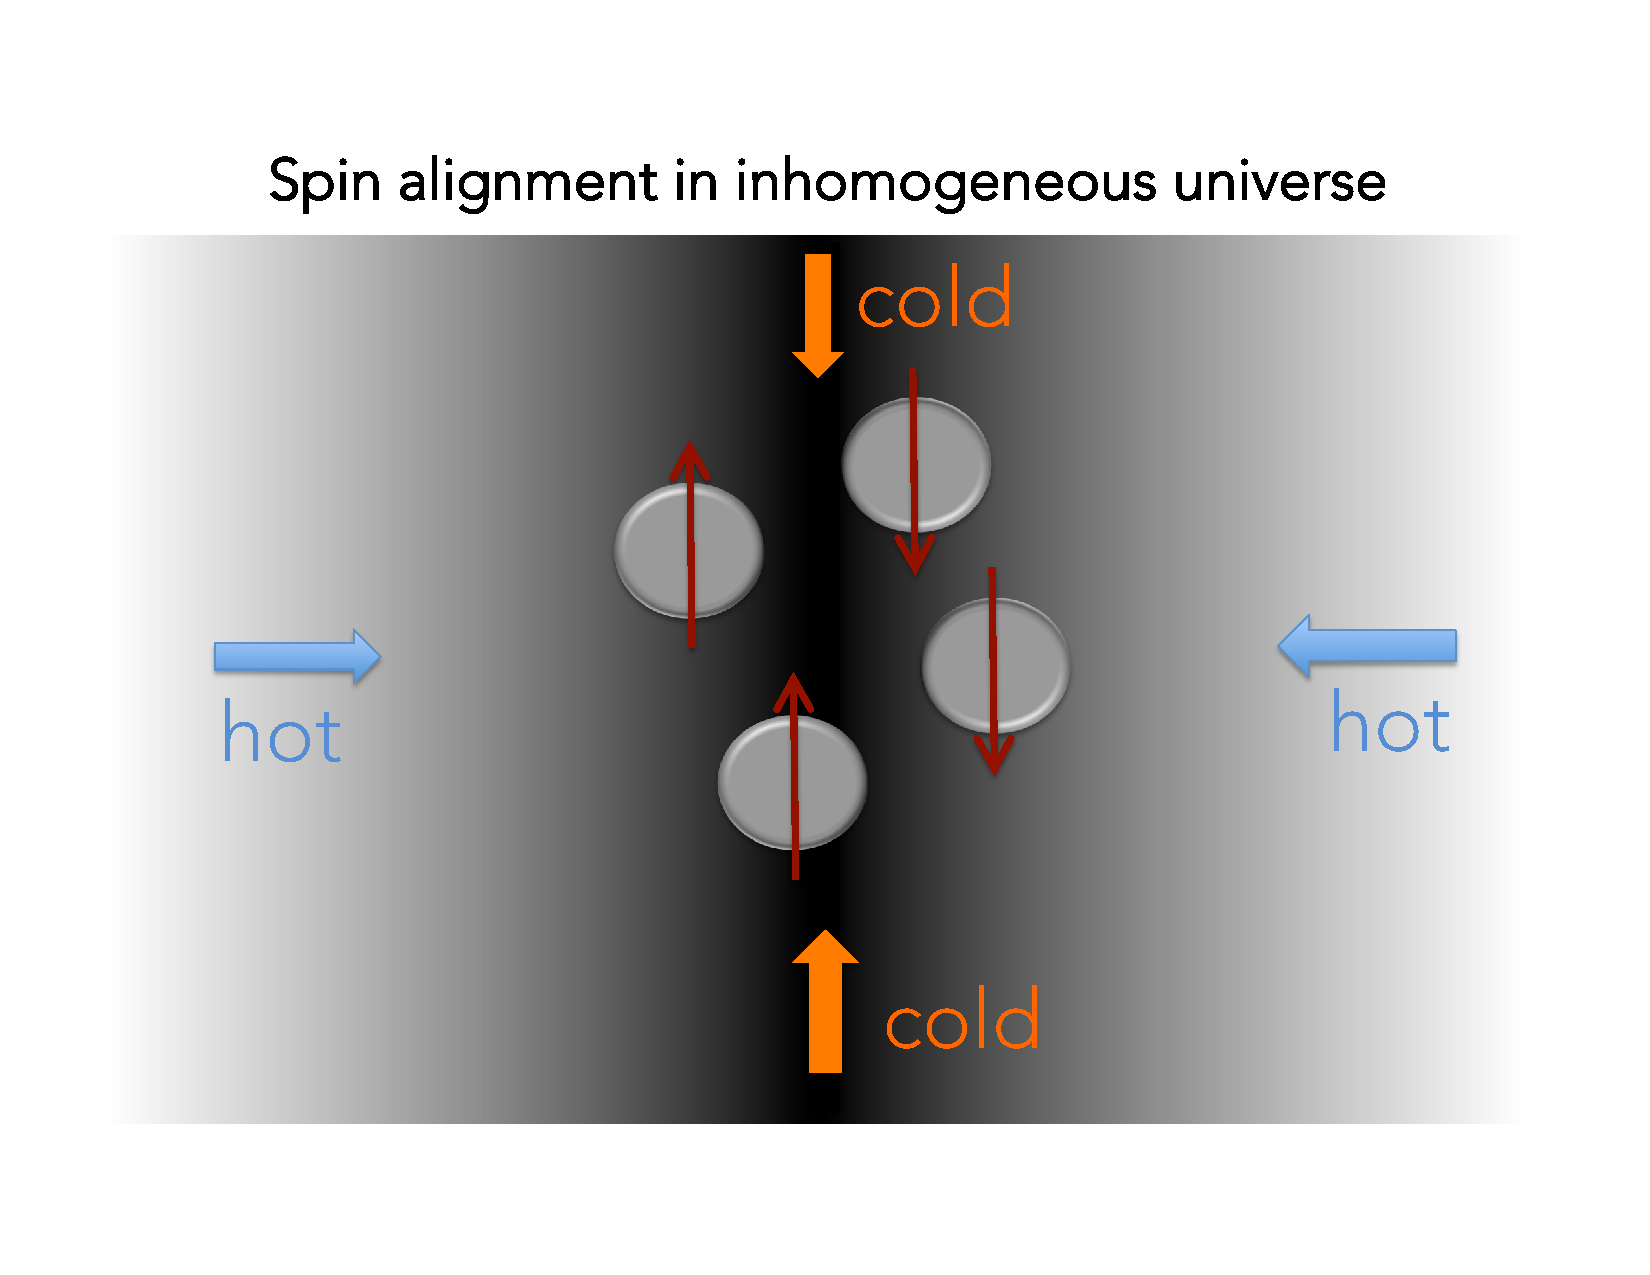
\includegraphics[width=.45\textwidth,keepaspectratio=true]{spin_aligned.pdf}
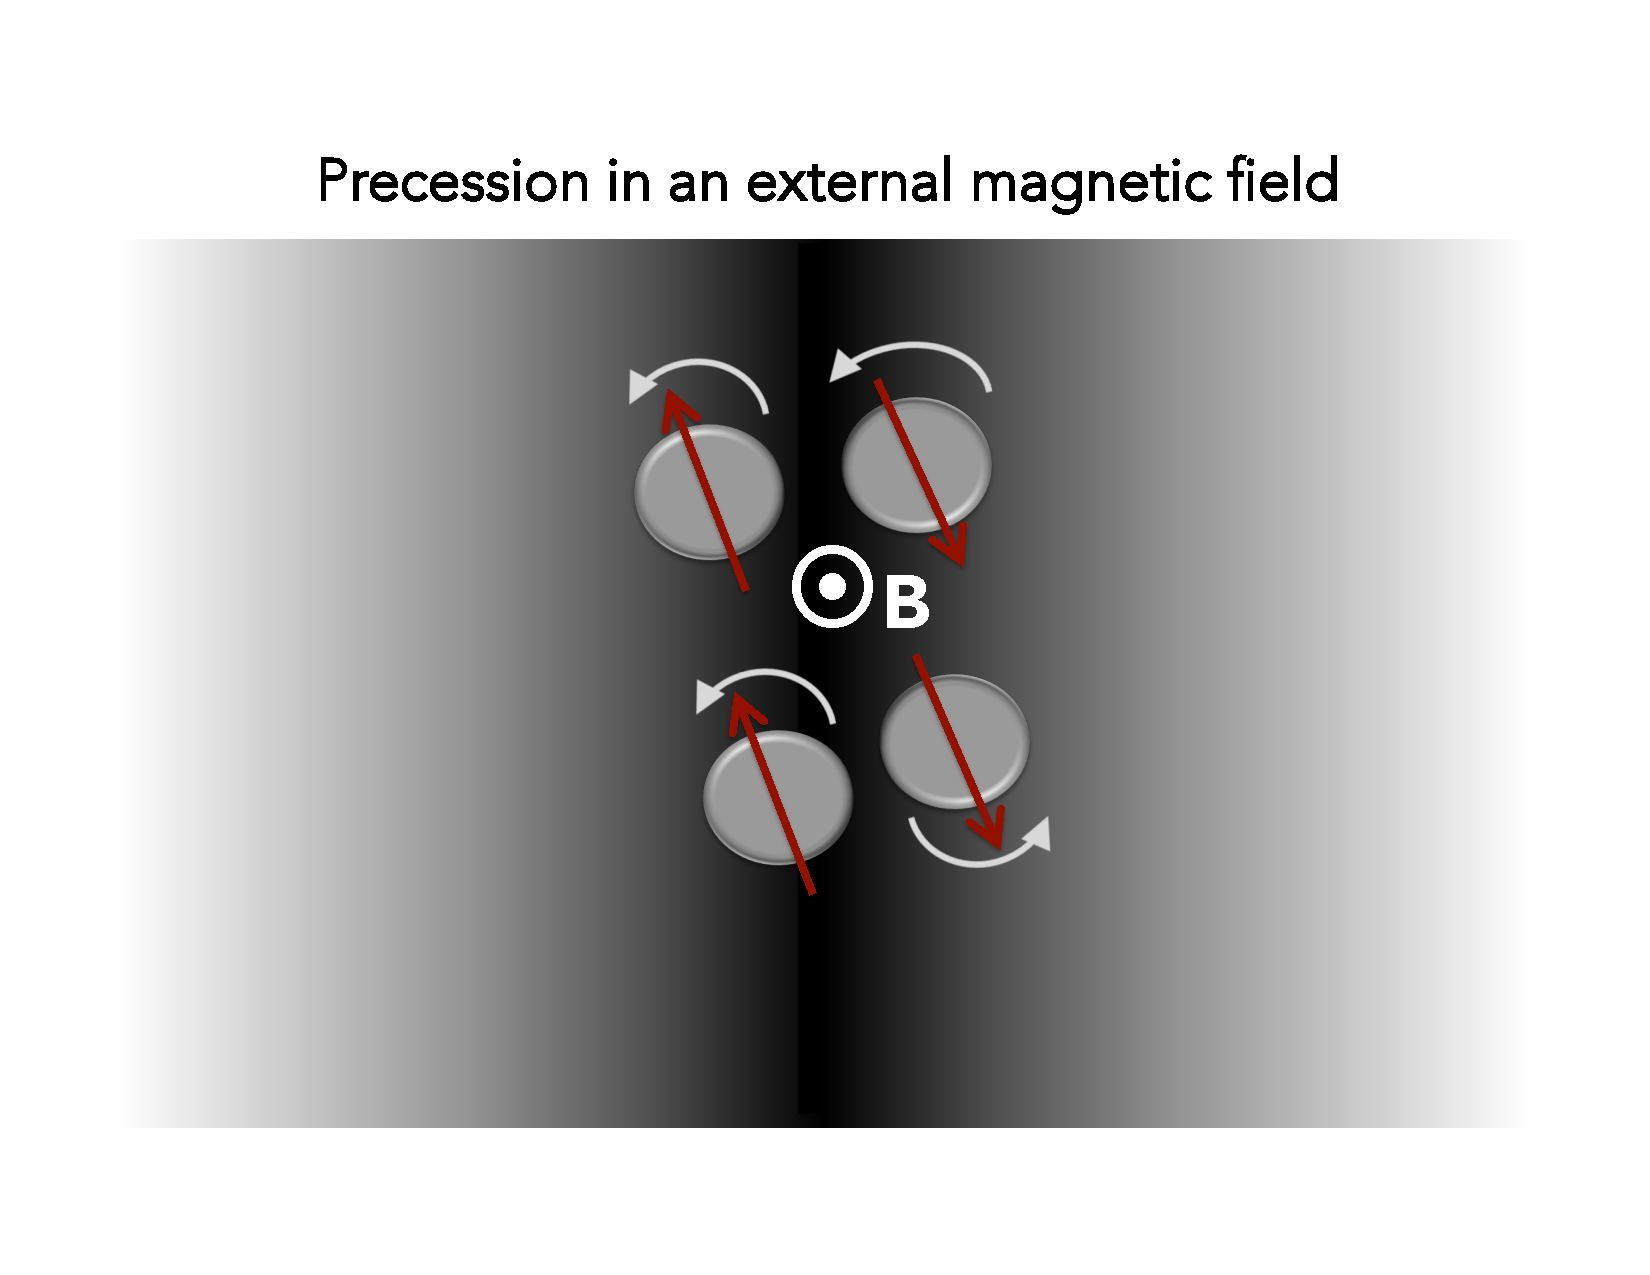
\includegraphics[width=.45\textwidth,keepaspectratio=true]{precession.pdf}
\caption{Illustration of the effect of a magnetic field on hydrogen atoms in the excited state of 21--cm transition in cosmological setting. In the classical picture, magnetic moments of the atoms (depicted as red arrows) are aligned with density gradients (see upper panel; the gradient is depicted with the background shading), unless they precess about the direction of ambient magnetic field (pointing out of the page on the lower panel). When the precessing atoms decay back into the ground state, the emitted quadrupole (aligned with the direction of the magnetic moments) is misaligned with the incident quadrupole. This offset can be observed as a statistical anisotropy in 21--cm brightness--temperature signal, and used to trace cosmological magnetic fields.\label{fig:precession}}
\end{figure}
Magnetic moments of hydrogen atoms in the excited (triplet) state of the 21--cm line transition tend to align with the incident quadrupole of the 21--cm radiation from the surrounding medium. This effect of ``ground--state alignment'' \cite{Yan08,Yan12} arises in a cosmological setting due to velocity--field gradients. In the presence of an external magnetic field, the emitted 21--cm quadrupole is misaligned with the incident quadrupole, due to atomic precession; this is illustrated in Fig.~\ref{fig:precession}. The resulting emission anisotropy can be used to trace magnetic fields at high redshifts.

The main result of Paper I was derivation of the 21--cm brightness--temperature fluctuation\footnote{Standard notation, used in other literature and in Paper I of this series, for this quantity is $\delta T_b$; however, we use $T$ here to simplify our expressions.} $T_{\rm }$, including the effects of magnetic precession, as a function of the line--of--sight direction ${\bf{\widehat n}}$, 
\beq
\bga
   T_{\rm }({\bf{\widehat n}}, {{\vec k}}) = \left( 1 - \frac{T_\gamma}{T_{\rm s}} \right) x_{1{\rm s}} \left( \frac{1+z}{10} \right)^{1/2} \\
  \times \biggl[ 26.4 \ {\rm mK} \Bigl\{ 1 + \left(1 + ({\bf{\widehat k}} \cdot {\bf{\widehat n}})^2 \right)\delta(\vec k) \Bigr\}  
- 0.128 \ {\rm mK} \left( \frac{T_\gamma}{T_{\rm s}} \right)\\ \times x_{1{\rm s}} \left( \frac{1+z}{10} \right)^{1/2}  
 \Bigl\{ 1 + 2 \left(1 + ({\bf{\widehat k}} \cdot {\bf{\widehat n}})^2 \right)\delta(\vec k) \\
- \frac{ \delta(\vec k) }{15} \sum_m \frac{4\pi}{5} \frac{Y_{2 m}({\bf{\widehat k}}) \left[ Y_{2 m} ({\bf{\widehat n}}) \right]^* }{1 + x_{ \alpha, (2) } + x_{{\rm c}, (2)} - i m x_{\rm B}} \Bigr\} \biggr] \mbox{,} 
\ega
\label{eq:tbsoln}
\eeq
where the magnetic field is along the $z$ axis in the rest frame of the emitting atoms (in which the spin--zero spherical harmonics $Y_{2 m}$ are defined in the usual way); $\delta(\vec k)$ is a density--fluctuation Fourier mode corresponding to the wave vector $\vec k$ whose direction is along the unit vector $\bf{\widehat k}$; $x_{\alpha, (2)}$, $x_{{\rm c}, (2)}$, and $x_{\rm B}$ parametrize the rates of depolarization of the ground state by optical pumping and atomic collisions, and the rate of magnetic precession (relative to radiative depolarization), respectively (defined in detail in Paper I), and are all functions of redshift $z$; $T_{\rm s}$ and $T_\gamma$ are the spin temperature and the CMB temperature at redshift $z$, respectively. Fig.~\ref{fig:hp} illustrates the effect of the magnetic field on the brightness temperature emission pattern in the frame of the emitting atoms; shown are the quadrupole patterns corresponding to the last term of \eq{\ref{eq:tbsoln}}, for various strengths of the magnetic field. Notice that there is a saturation limit for the field strength---for a strong field, the precession is much faster than the decay of the excited state of the forbidden transition, and the emission pattern asymptotes to the one shown in the bottom panel of Fig.~\ref{fig:hp}. Above this limit, the signal cannot be used to reconstruct the strength of the field. However, in this ``saturated regime'', it is still possible to distinguish the presence of a strong magnetic field from the case of no magnetic field, as we discuss in detail in \S\ref{sec:fisher}.
\begin{figure}
\centering
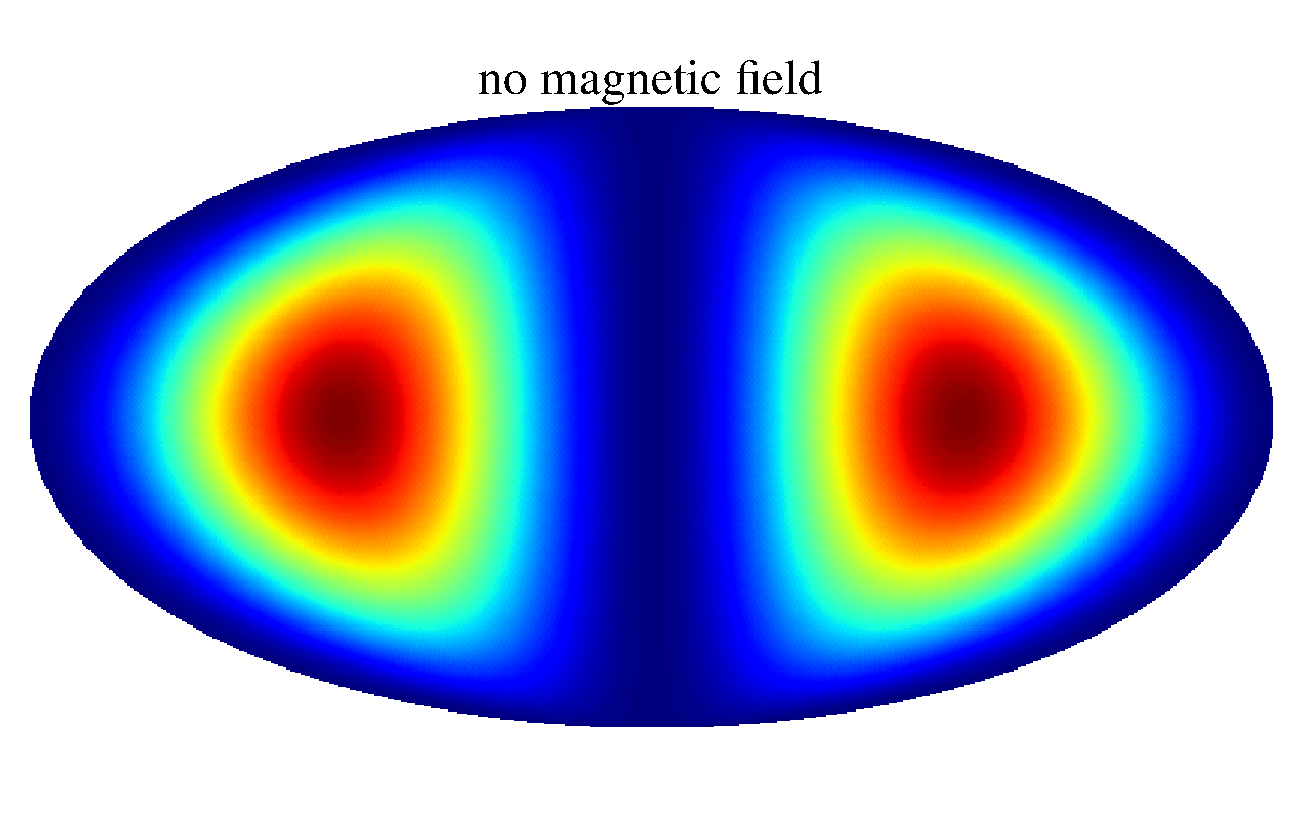
\includegraphics[width=.4\textwidth,keepaspectratio=true]{hp_B_0e+00G.pdf}
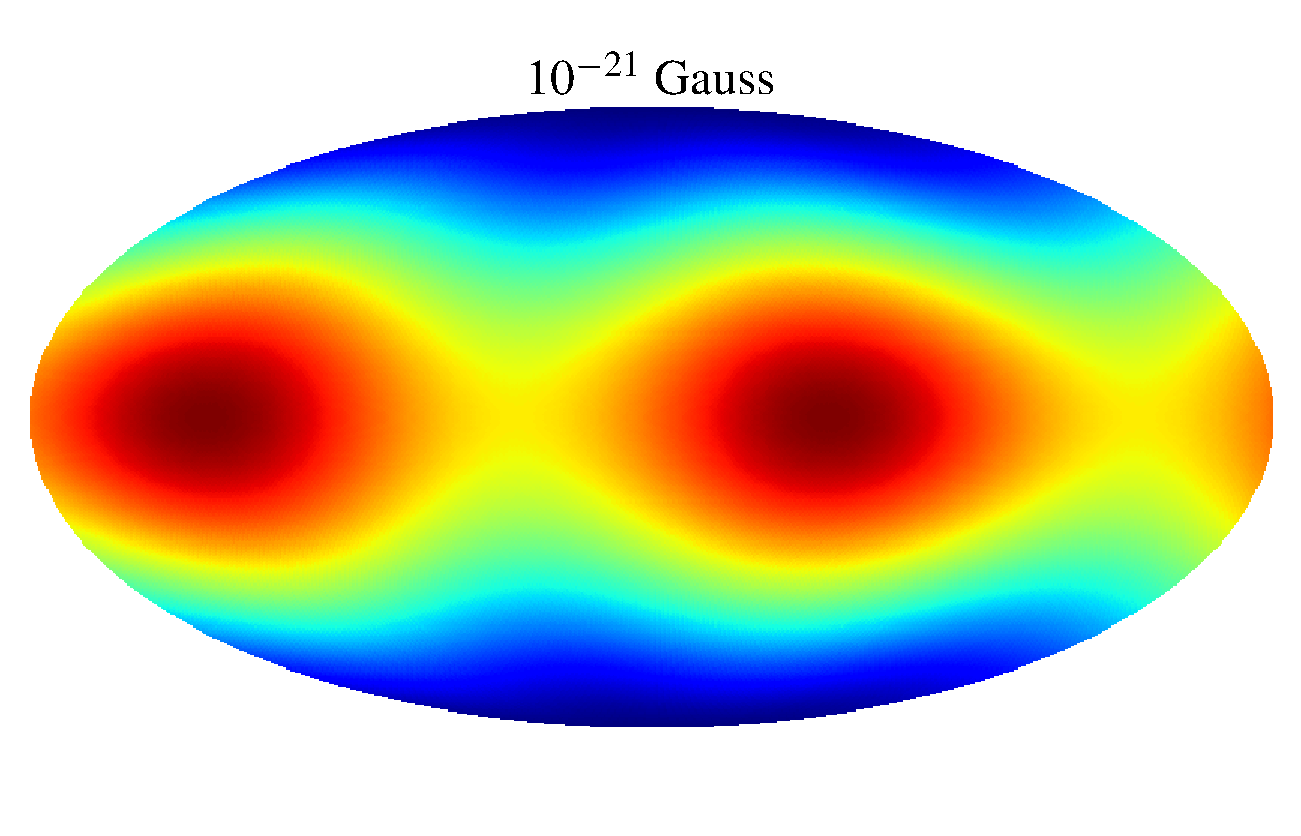
\includegraphics[width=.4\textwidth,keepaspectratio=true]{hp_B_1e-18G.pdf}
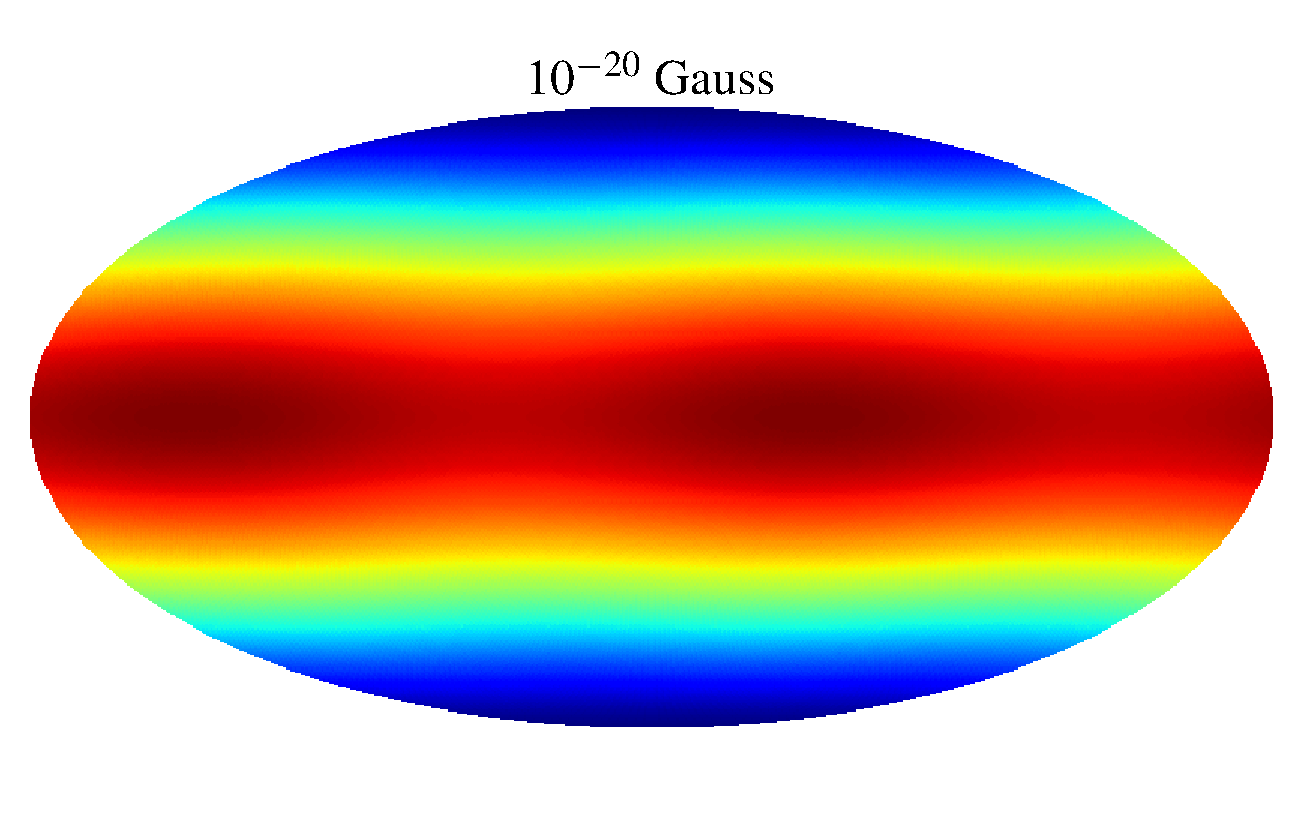
\includegraphics[width=.4\textwidth,keepaspectratio=true]{hp_B_1e-17G.pdf}
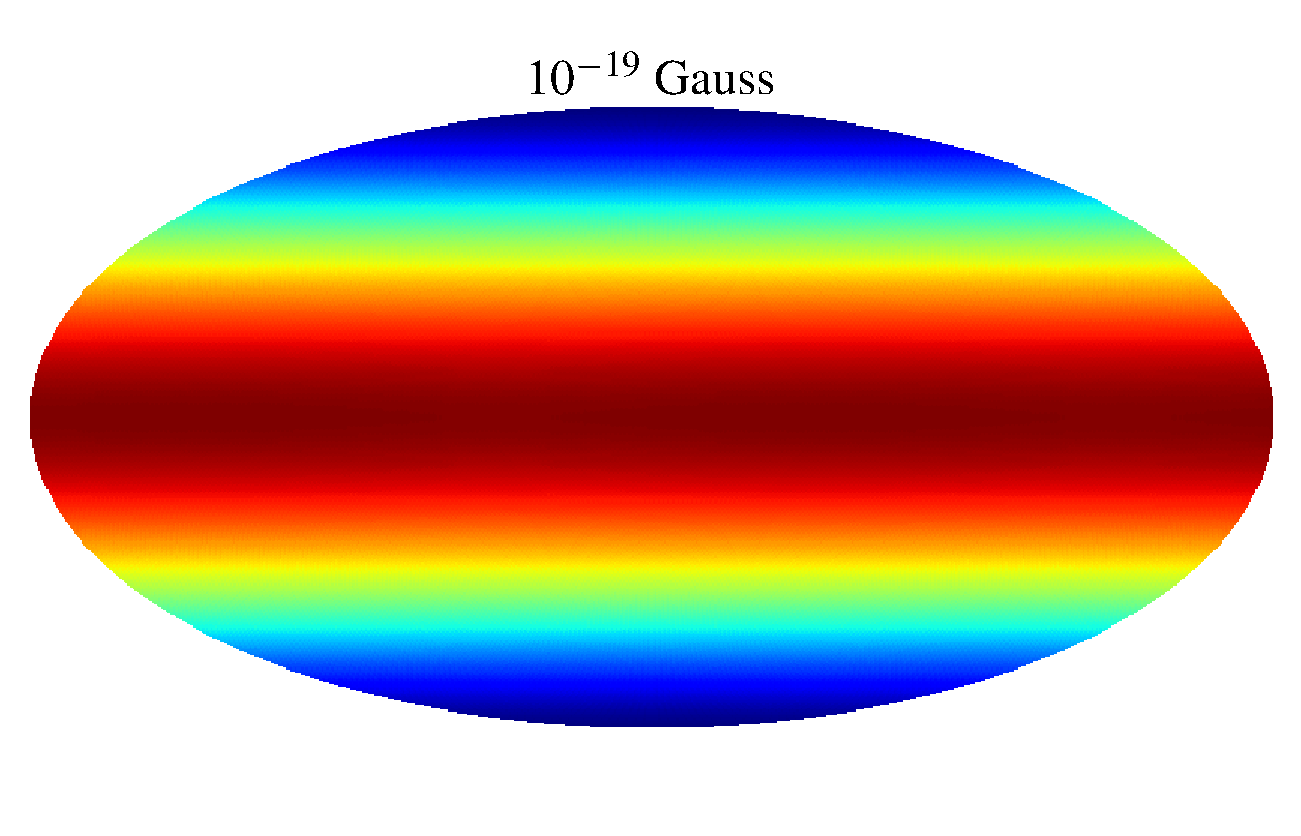
\includegraphics[width=.4\textwidth,keepaspectratio=true]{hp_B_1e-16G.pdf}
\caption{Illustration of the quadrupolar pattern of 21--cm emission from the last ($\vec B$--dependent) term of \eq{\ref{eq:tbsoln}} in the frame of the emitting atoms, shown in Molleweide projection, where the intensity increases from blue to red shades. This illustration in all panels shows the case where $\vec k$ matches the direction of the hot spots in the top panel, and is perpendicular to the direction of the magnetic field (along the vertical axis in all panels). Every pixel in the maps corresponds to a unique direction $\bf{\widehat n}$ in Eq.~(\ref{eq:tbsoln}). Lower panels correspond to increasingly stronger magnetic field (strength denoted on each panel in comoving units, for $z=21$), with the bottom panel corresponding to the saturated case. Notice how the type of quadrupole in the top panel (weak--field regime) is distinct from that in the bottom panel (saturated regime). \label{fig:hp}}
\end{figure}

The effect of quadrupole misalignment arises at second order in optical depth (it is a result of a two--scattering process), and is thus a small correction to the total brightness--temperature fluctuation. However, owing to the long lifetime of the excited state of the forbidden transition (during which even an extremely slow precession can have a large cumulative effect on the direction of the quadrupole, at second order), the misalignment is exquisitely sensitive to magnetic fields in the IGM at redshifts prior to cosmic reionization. As we showed in Paper I, a minuscule magnetic field of  $10^{-21}$ Gauss (in comoving units) produces order--one changes in the direction of the quadrupole. This implies that a high--precision measurement of the 21--cm brightness--temperature two--point correlation function intrinsically has that level of sensitivity to magnetic fields prior to the epoch of reionization (when most of the IGM is still neutral). We now proceed to develop a formalism to search for magnetic fields at high redshifts using this effect, and to forecast the sensitivity of future 21--cm experiments. 